%%%%%%%%%%%%%%%%%%%%%%%%%%%%%%%%%%%%%%%%%
% Journal Article
% LaTeX Template
% Version 1.4 (15/5/16)
%
% This template has been downloaded from:
% http://www.LaTeXTemplates.com
%
% Original author:
% Frits Wenneker (http://www.howtotex.com) with extensive modifications by
% Vel (vel@LaTeXTemplates.com)
%
% License:
% CC BY-NC-SA 3.0 (http://creativecommons.org/licenses/by-nc-sa/3.0/)
%
%%%%%%%%%%%%%%%%%%%%%%%%%%%%%%%%%%%%%%%%%

%----------------------------------------------------------------------------------------
%	PACKAGES AND OTHER DOCUMENT CONFIGURATIONS
%----------------------------------------------------------------------------------------

\documentclass[twoside,twocolumn,paper=letter]{article}
\usepackage[cm]{fullpage} 

\usepackage{blindtext} % Package to generate dummy text throughout this template 

\usepackage[sc]{mathpazo} % Use the Palatino font
\usepackage[T1]{fontenc} % Use 8-bit encoding that has 256 glyphs
\linespread{1.05} % Line spacing - Palatino needs more space between lines
\setlength\parindent{0pt}
\usepackage[protrusion=true,expansion=true]{microtype} % Slightly tweak font spacing for aesthetics

\usepackage[english]{babel} % Language hyphenation and typographical rules

%\usepackage[hmarginratio=1:1,top=32mm,columnsep=20pt]{geometry} % Document margins
\usepackage[hang, small,labelfont=bf,up,textfont=it,up]{caption} % Custom captions under/above floats in tables or figures
\usepackage{booktabs} % Horizontal rules in tables

\usepackage{lettrine} % The lettrine is the first enlarged letter at the beginning of the text

\usepackage{enumitem} % Customized lists
\setlist[itemize]{noitemsep} % Make itemize lists more compact

\usepackage{abstract} % Allows abstract customization
\renewcommand{\abstractnamefont}{\normalfont\bfseries} % Set the "Abstract" text to bold
\renewcommand{\abstracttextfont}{\normalfont\small\itshape} % Set the abstract itself to small italic text

\usepackage{titlesec} % Allows customization of titles
\renewcommand\thesection{\Roman{section}} % Roman numerals for the sections
\renewcommand\thesubsection{\roman{subsection}} % roman numerals for subsections
\titleformat{\section}[block]{\large\scshape\centering}{\thesection.}{1em}{} % Change the look of the section titles
\titleformat{\subsection}[block]{\large}{\thesubsection.}{1em}{} % Change the look of the section titles

\usepackage{fancyhdr} % Headers and footers
\pagestyle{fancy} % All pages have headers and footers
\fancyhead{} % Blank out the default header
\fancyfoot{} % Blank out the default footer
%\fancyhead[C]{Running title $\bullet$ May 2016 $\bullet$ Vol. XXI, No. 1} % Custom header text
\fancyfoot[RO,LE]{\thepage} % Custom footer text

\usepackage{titling} % Customizing the title section

\usepackage{hyperref} % For hyperlinks in the PDF
\usepackage{graphicx} % Including graphics
\usepackage{subcaption} % Including subfigures
\usepackage{stfloats} 
%----------------------------------------------------------------------------------------
%	TITLE SECTION
%----------------------------------------------------------------------------------------

\setlength{\droptitle}{-4\baselineskip} % Move the title up

\pretitle{\begin{center}\Large\bfseries} % Article title formatting
\posttitle{\end{center}} % Article title closing formatting
\title{Applying Machine Learning to Predict and Explain Primate Consortship} % Article title
\author{%
\textsc{Josh King} \\[1ex] 
\and 
\textsc{Vayu Kishore} \\[1ex] 
\and 
\textsc{Filippo Ranalli} \\[1ex] 
}
\date{} % Leave empty to omit a date
\renewcommand{\maketitlehookd}{%
%\begin{abstract}
%\noindent \blindtext % Dummy abstract text - replace \blindtext with your abstract text
%\end{abstract}
}

%----------------------------------------------------------------------------------------

\begin{document}

% Print the title
\maketitle

%----------------------------------------------------------------------------------------
%	ARTICLE CONTENTS
%----------------------------------------------------------------------------------------

\section{Introduction}

\lettrine[nindent=0em,lines=3]{T} he mating behavior of a species drives genetic
interchange and is a major driver of evolution within populations. Factors that
contribute to consortship may range from genetic causes, such as physical traits
expressed due to the presence of a gene, to those that are social or behavioral.
The contribution of social factors is of particular interest for animals that
live in structured groups, where factors such as rank within a social heirarchy
may impact mating success.  Investigating this topic will provide deeper insight
into the factors of mating success in social mammals, which may be extended to
apply to humans as well.\\

We apply machine learning methods to investigate the behavioral and genetic
reasons for success and failure of mating between wild baboon pairs. Our
analysis applies machine learning methods to examine whether successful
consortships can be predicted, and whether certain behavioral or genetic
features are especially relevant in determining consortship. Additionally, we
investigate whether successful and unsuccessful pairs can be clustered, and
whether there are certain clusters present in one group that are not present in
the other.

%------------------------------------------------

\section{Related Work}

\cite{Tung:2012} examine the impact of behavioral and genetic effects on
consortship in male/female baboon pairs in a wild yellow baboon population. They
found that a mix of both genetic and social factors drive non-random mating
within populations.

\section{Dataset}
The dataset that we use was collected and analyzed using statistical methods by
\cite{Tung:2012}. It contains observations about the success of potential baboon
mating pairs. In particular, it specifies if , male/female baboon pairings were
successful in consorting when given the opportunity.  There are approximately
12,000 observations, and the features are a mix of behavioral data such as the
rank difference between the male and female pair, as well as genetic data, such
as the estimated genetic distance between the pair. 
\subsection{Features}
There are several categories of features present within the dataset.
\begin{itemize}
  \item{\textbf{Observed biological and genetic features}: These include female age
    and conceptiveness, as well as the estimated genetic diversity and genetic
    distance between the mating pair.}
  \item{\textbf{Observed behavioral features}: These include rank of the mating pair
    within the social heirarchy of the group and how many males and females from
    their group were present when the interaction of the pair took place.}
  \item{\textbf{Derived Pairwise Features}: Some features are
    transformations applied to the observed features described above, which were
    computed by \cite{Tung:2012}. Some of the transformations compute a pairwise
    score based on a combination of the male and female attributes. For example,
    the rank\_interact feature represents the combination of male and female
    ranks.
    }
  \item{\textbf{Derived Single Features}: The remaining features are single
    raw features which are scaled based on an assumed distribution.  The
    male\_rank\_transform feature, for example, scales the male rank based on an
    exponential distribution.}
\end{itemize}

In addition to the different categories, some of the features, such as
(untransformed) rank, are ordinal, while others, such as estimated genetic
distance are real-valued.

\subsection{Identifiers and Labels}
Each datapoint contains an identifier of the male and female pair in an
interaction that could lead to a consortship and a 0/1 label which indicates
whether the male and female consorted.

\section{Preprocessing}

In the analysis that we have conducted up to this point, we have not performed
any preprocessing on the data. We may consider applying additional
transformations to the features, such as whitening using PCA if we find that our
models are negatively impacted by the colinearity between features.

\section{Methods}
\subsection{Materials}

To perform our analysis, we used the \texttt{scikit-learn} python package. Methods
that were not readily available in \texttt{scikit-learn}, such as feature selection, were
implemented independently in python.


\subsection{Classification}
% feature selection
% algos and cross-validation
One of the very first things we thought critical in understanding the data was running a range of classifiers and visualizing which ones would perform best according to a set of metrics. However, classification on the training set alone does not yield a significant portrait of the data, hence we opted to perform K-fold validation 
on linear and non-linear classifiers, each embedded in a forward and backward feature selection algorithm framework.\\

The linear classifiers examined are logistic regression and linear SVM, while the non-linear classifiers are gaussian and polynomial SVM. For each algorithm, we tuned the hyper-parameters (i.e. the regularization) and we ensured that the class weights were balanced, given that the negative (non-consort) labels outweigh the positive labels (consort) by 5-to-1. When performing K-fold validation with 4 folds, the data was randomly shuffled so as to avoid positive labels concentrating in a particular training or test set, biasing the performance. Moreover, for each algorithm and feature subset we evaluated the error, precision, recall and F1 score as an average on each of the K-cluster training and test sets. Finally we stored the confusion matrix, obtained by running 75-25 hold-out cross-validation with all the features and for the models that performed best.
\subsection{Clustering}
% kmeans on non-consort pairs, examined centroids, used PCA to visualize

We ran the k-means algorithm with 4 clusters on the consorting and
non-consorting pairs. To visualize the clusters, we then used dimensionality
reduction techniques such as PCA and t-SNE manifold tool.\\

We also examined using affinity propagation which can automatically determine
the number of clusters.

\subsection{Graphical Approach}

%------------------------------------------------
One approach to this problem is to use the interactions as edges and the baboons as nodes. Due to only heterosexual interactions occurring this means that the resulting graph is bipartite. The classification then becomes  an edge prediction task. Most previous work on this has been on just predicting whether or not edges exist, not predicting the label of the edge. We adapted current methods to predict the label of an edge rather than whether or not it exists. \\
\cite{Macskassy:2007} use a simple method that computes the similarities of the attributes of nodes to determine the weight of latent edges between nodes. Because most of the attributes are not inherent to the baboons, but are depdendent on the scenario in which interactions occur we adapt this method to look at the similarity between the proposed edge and already existing edges between those two nodes. More formally, if there is some set of nodes $V$ and some set of edges $E$ where each edge $e_i$ has some associated features $f_i$ and some associated label $l_i\in \{0,1\}$ then to determine the label of a new edge $e_n$ between nodes $u$ and $v$ we would compute 
$$argmax_{label \in \{0,1\}} \frac{\sum_{e_i \in E}1\{l_i=label\}\cdot|e-e_n|_2}{\sum_{e_i \in E}1\{l_i=label\}}$$
We implemented this method, and also at a more specific method where instead of looking at all edges, we only look at edges where $u$ or $v$ are one of the endpoints of the edge. Both of these models end up being very similar to locally weighted regression so we implemented that and compare that also. \\

\section{Results and Discussion}
\subsection{Exploratory Data Analysis}
\begin{figure}
      \centering
          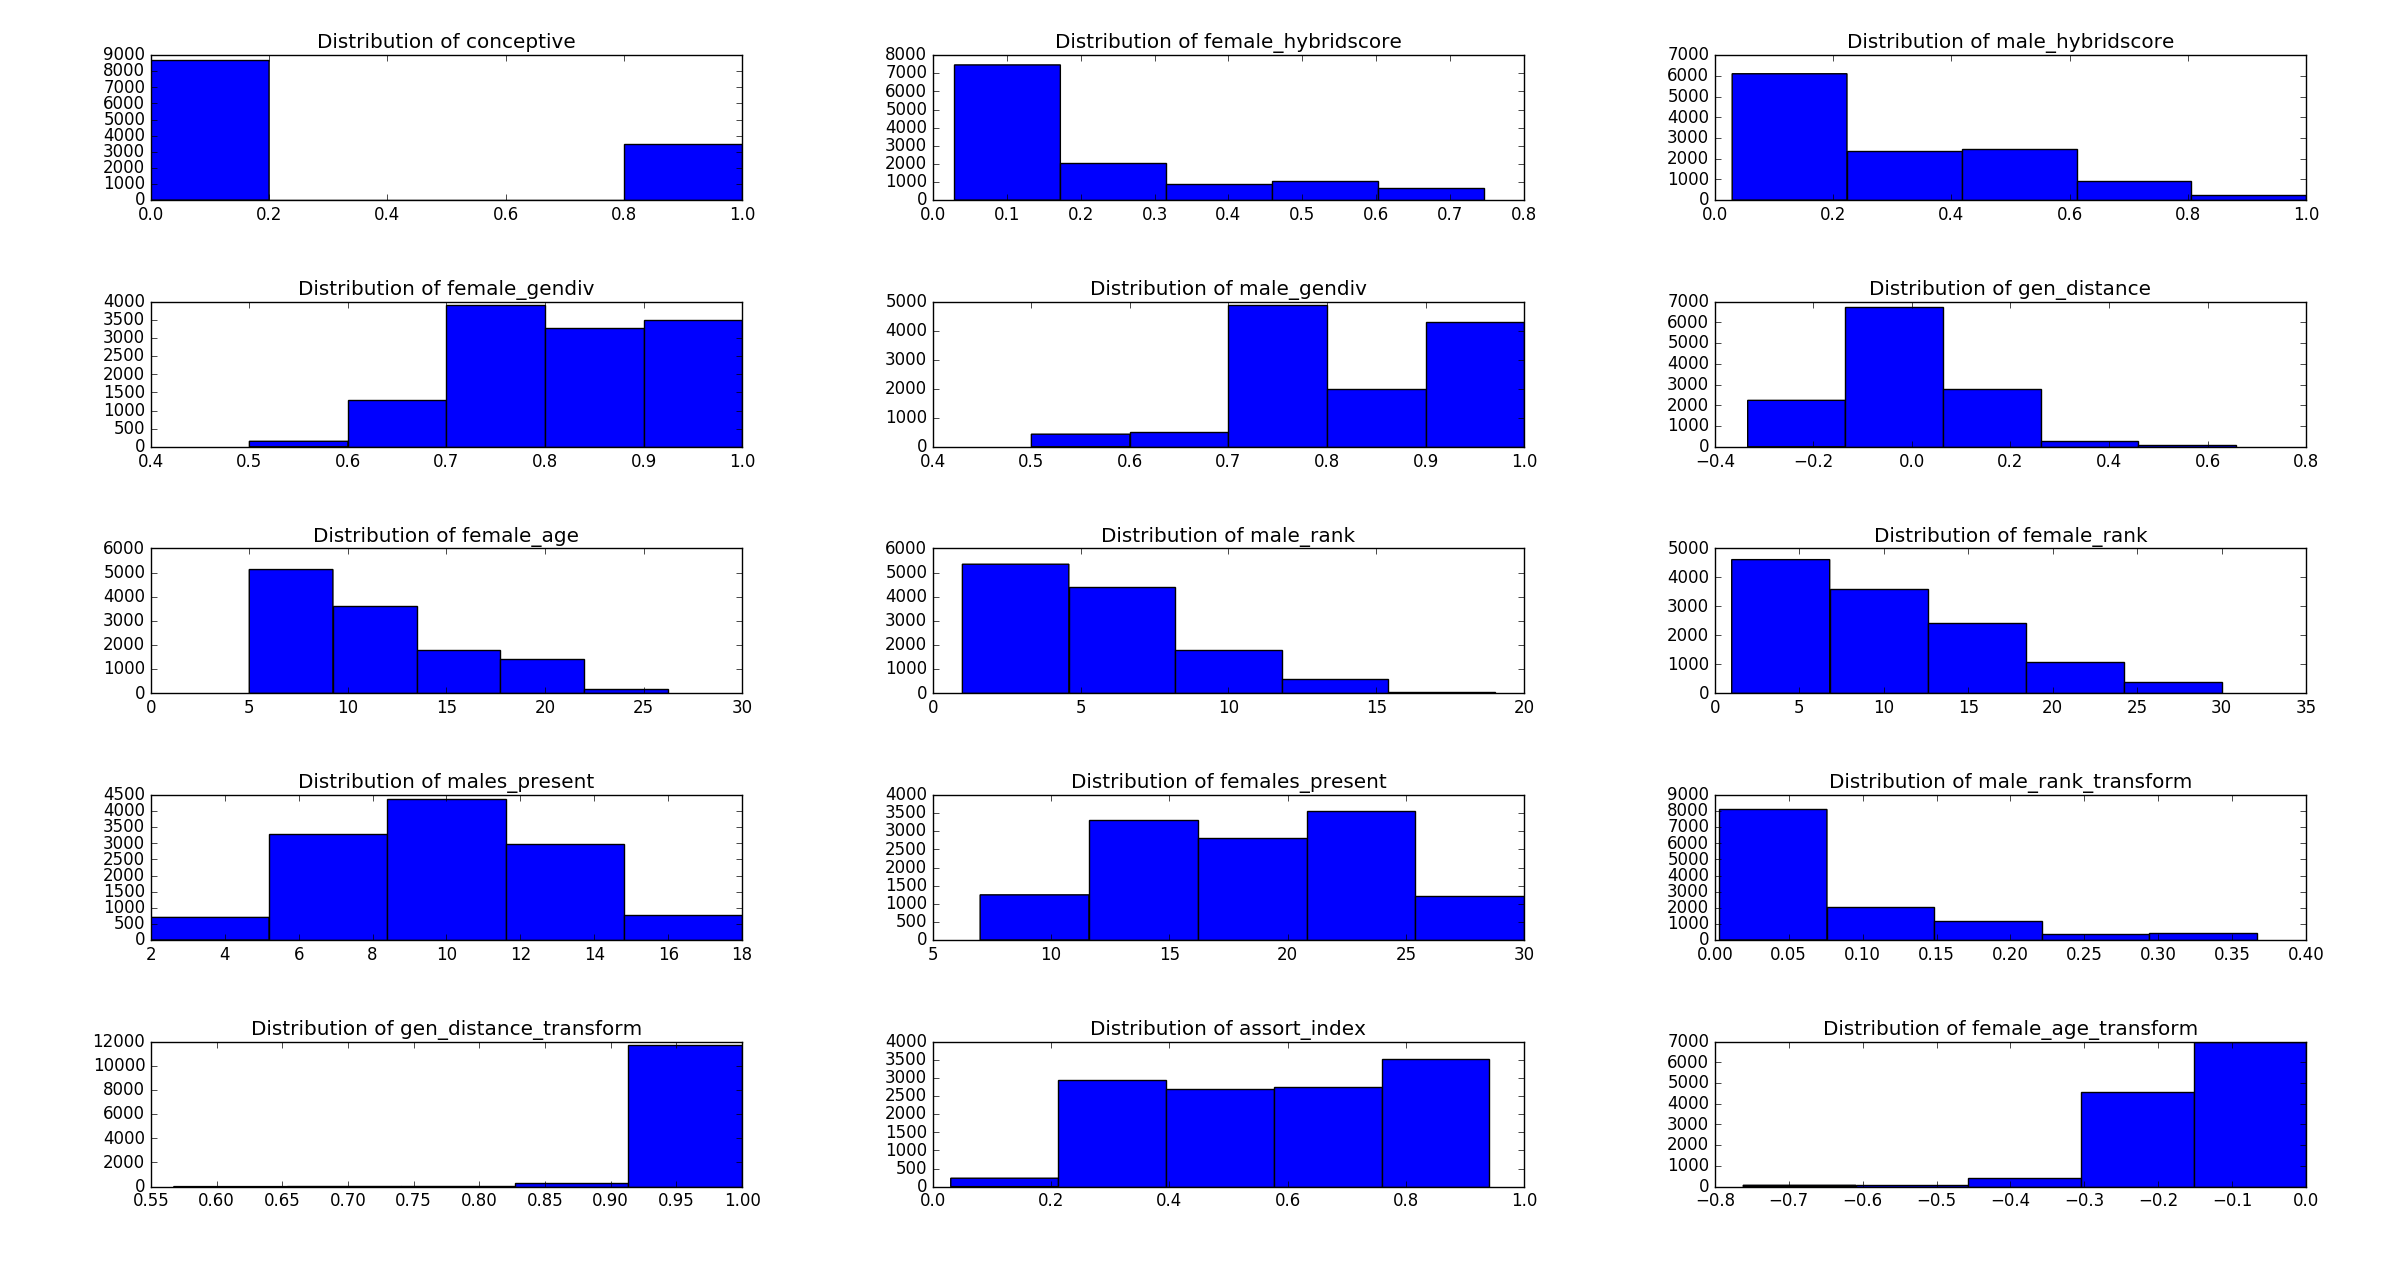
\includegraphics[width=0.5\textwidth]{../figs/all_feats_histogram.png}
  \caption{Distribution of features}
  \label{fig:figure_distrib}
\end{figure}
The features within the dataset seem to have varying distributions, as shown in
Figure \ref{fig:figure_distrib}. While some features, such as the number of
males present, seem to have a balanced distribution, others, such as the ages
and ranks, show a heavy skew with long tails.

\begin{figure}[h]
      \centering
          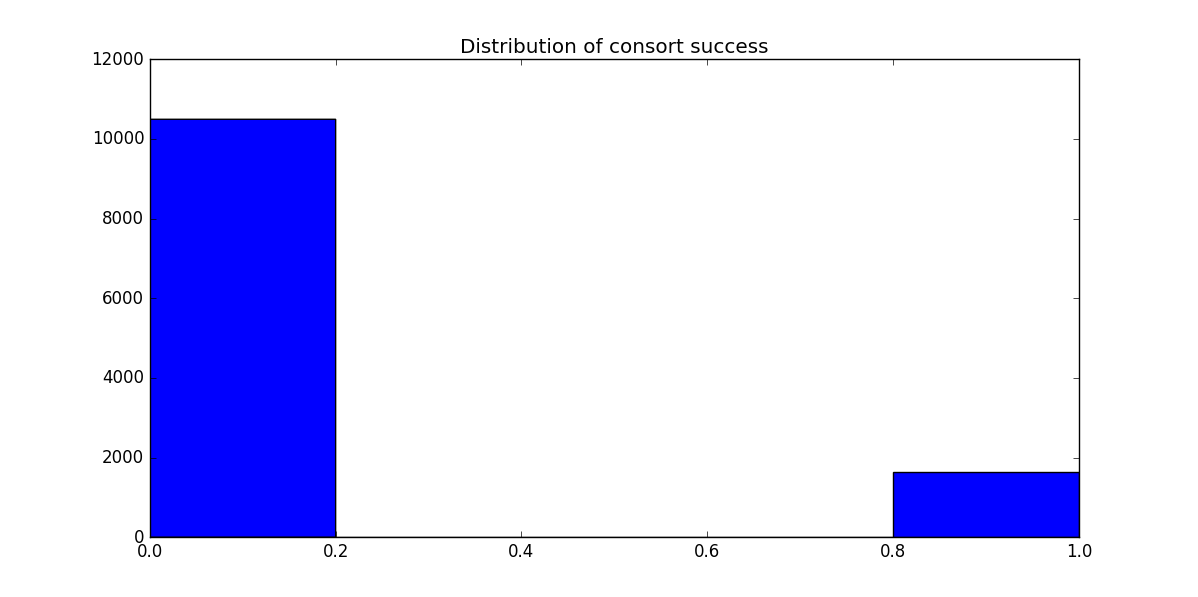
\includegraphics[width=0.5\textwidth]{../figs/consort_distrib.png}
  \caption{Distribution of consort/non-consort labels}
  \label{fig:label_distrib}
\end{figure}
Notably, we observe that the labels within the dataset are imbalanced -- there
are approximately ten times as many pairs which did not consort than those who
did. This imbalance may cause an issue in our classification algorithms since .
To avoid this we use the \texttt{weight} for \texttt{scikit-learn}'s classifiers
to automatically assign weights to the classes based on the incidence of
labels.\\
% PCA results
\begin{figure}
      \centering
          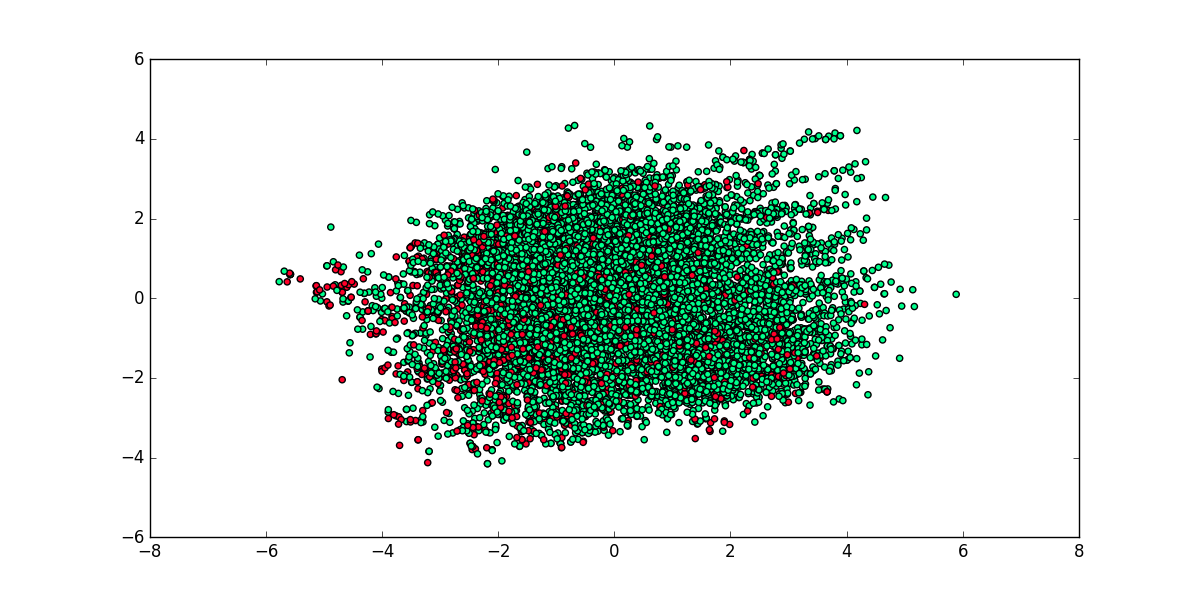
\includegraphics[width=0.5\textwidth]{../figs/consort_non_consort_visualization_pca.png}
  \caption{Reduced-dimensionality PCA visualization of consorting (red) and
  non-consorting pairs (green)}
  \label{fig:pca_vis}
\end{figure}
Using PCA to map higher dimensional dataset to 2 dimensions does not reveal
any lower-dimensional separation between the consorting/non-consorting pairs, as
shown in Figure \ref{fig:pca_vis}.
This indicates that the classification problem may be inherently
high-dimensional. The tSNE manifold mapping indicates this as well.
\subsection{Classification}
% confusion matrix

Running forward and backward feature selection shows that, for all the classifiers considered, the best performance in terms of the designated metrics is achieved when all the 16 derived and non-derived features are present. Moreover when breaking down the performance of each classifier, the top pick is gaussian SVM, followed by linear SVM. The metrics for the former algorithm are presented in the following table, along with the confusion matrices for the winner and the runner up. It is interesting to see how even though the gaussian SVM overall performs better in the metrics, linear SVM has a far higher rate of correct prediction on the positive labels. While the average errors with gaussian SVM are relatively high, the Fischer scores clearly showcase a poor weighed average of precision and recall, indicating this algorithm does not perform well.\\
\begin{figure}
      \centering
          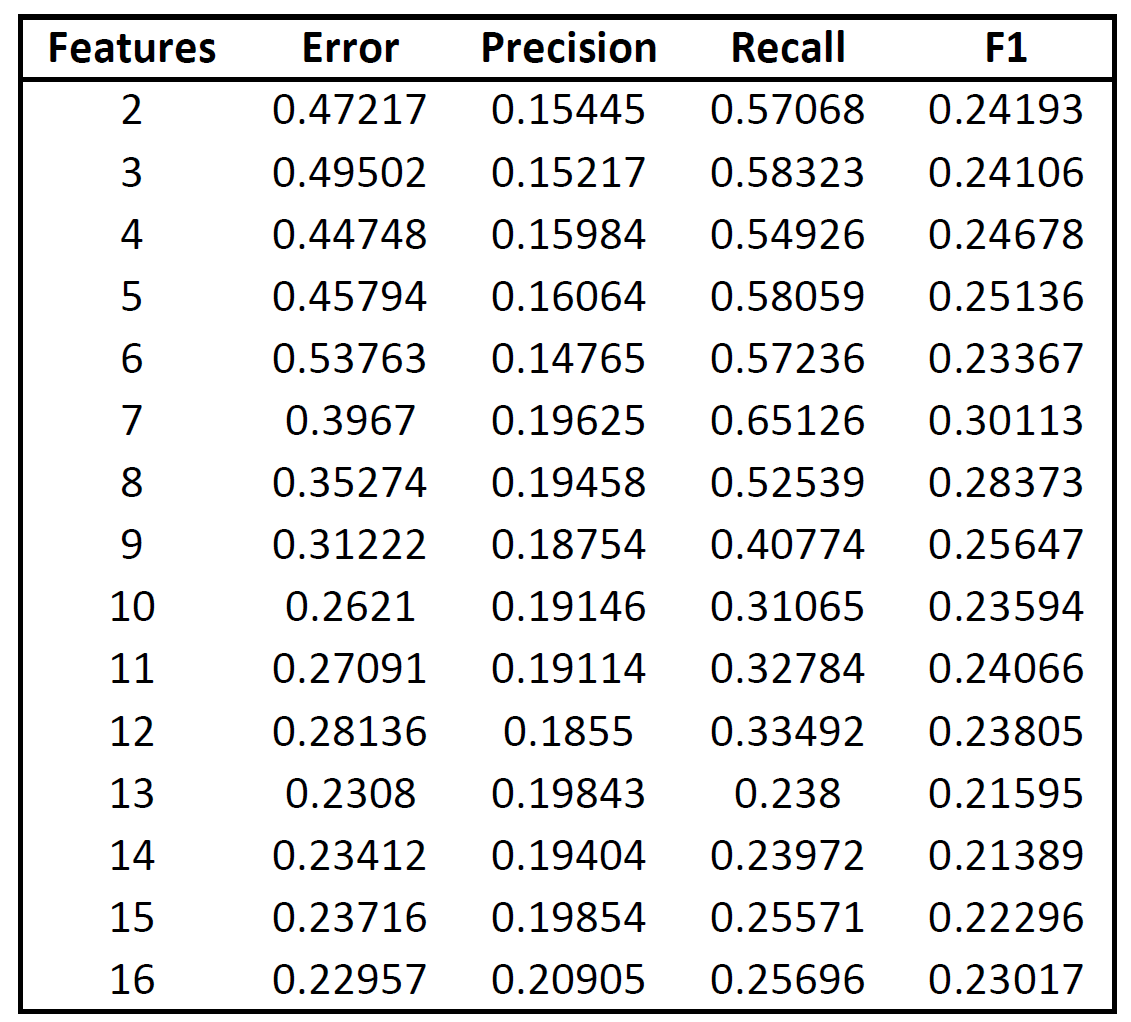
\includegraphics[width=0.5\textwidth]{../figs/ClassificationMetrics_RbfSVM.png}
  \caption{Gaussian SVM metrics based on number of features in forward feature selection.}
  \label{fig:rbf_svm_vis}
\end{figure}
\begin{figure}
      \centering
          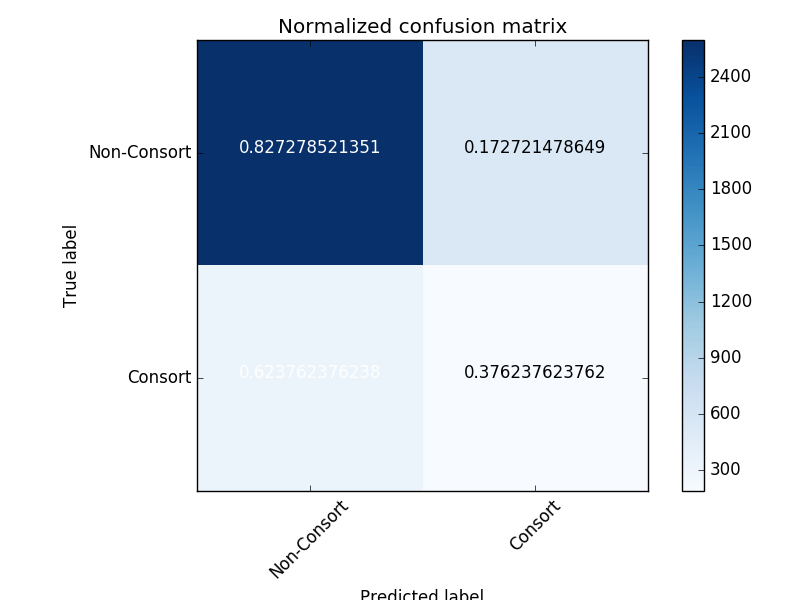
\includegraphics[width=0.5\textwidth]{../figs/gaussianSVM_CM.png}
  \caption{Gaussian SVM confusion matrix in 75-25 cross-validation.}
  \label{fig:cm_rbf_vis}
\end{figure}
\begin{figure}
      \centering
          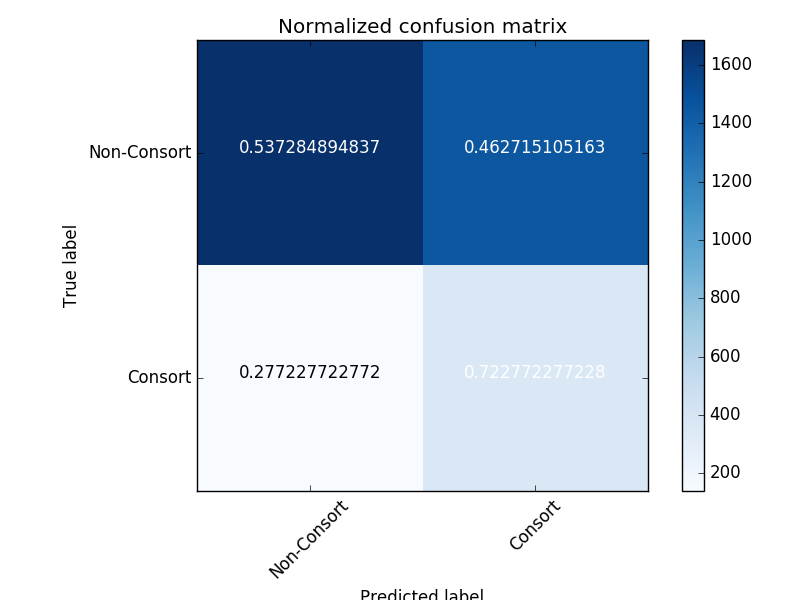
\includegraphics[width=0.5\textwidth]{../figs/linearSVM_CM.png}
  \caption{Linear SVM confusion matrix in 75-25 cross-validation.}
  \label{fig:cm_lin_vis}
\end{figure}


\subsection{Clustering}
% kmeans graphic
\begin{figure}[h]
      \centering
          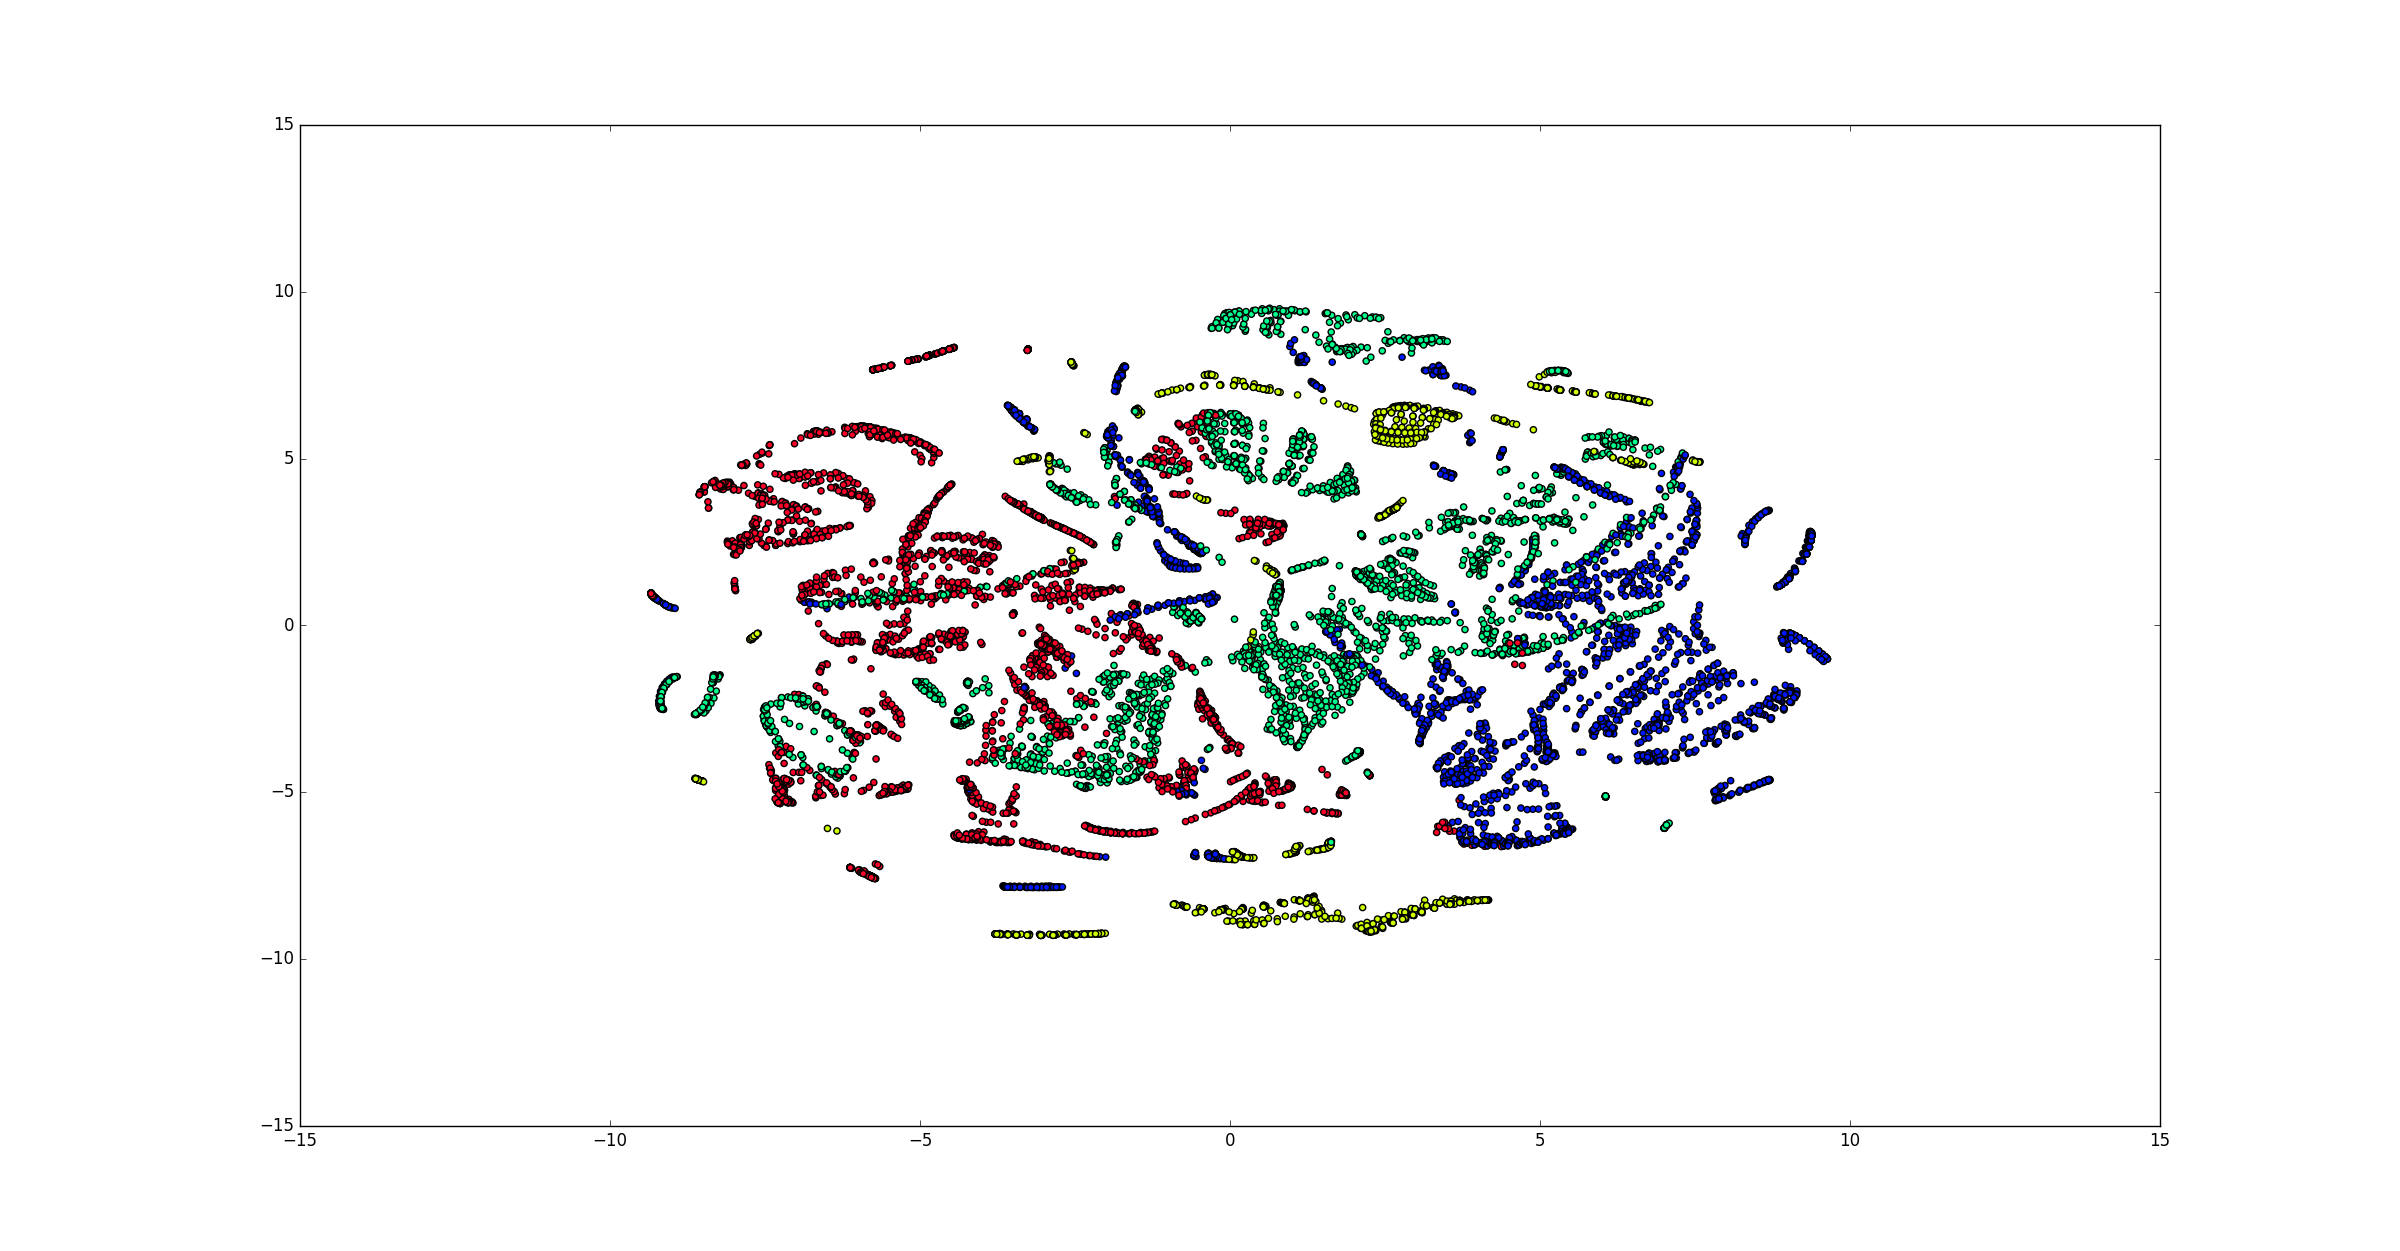
\includegraphics[width=0.5\textwidth]{../figs/non_consort_kmeans_2d_tsne.png}
  \caption{t-SNE visualization of K-Means with 4 clusters applied on consorting
  and non-consorting pairs.}
  \label{fig:non_consort_clustering_vis}
\end{figure}
Based on the centroids of the non-consorting clusters, non-consorting pairs can
be divided into:
\begin{itemize}
  \item{TODO: describe clusters}
\end{itemize}
\begin{figure}[h]
      \centering
          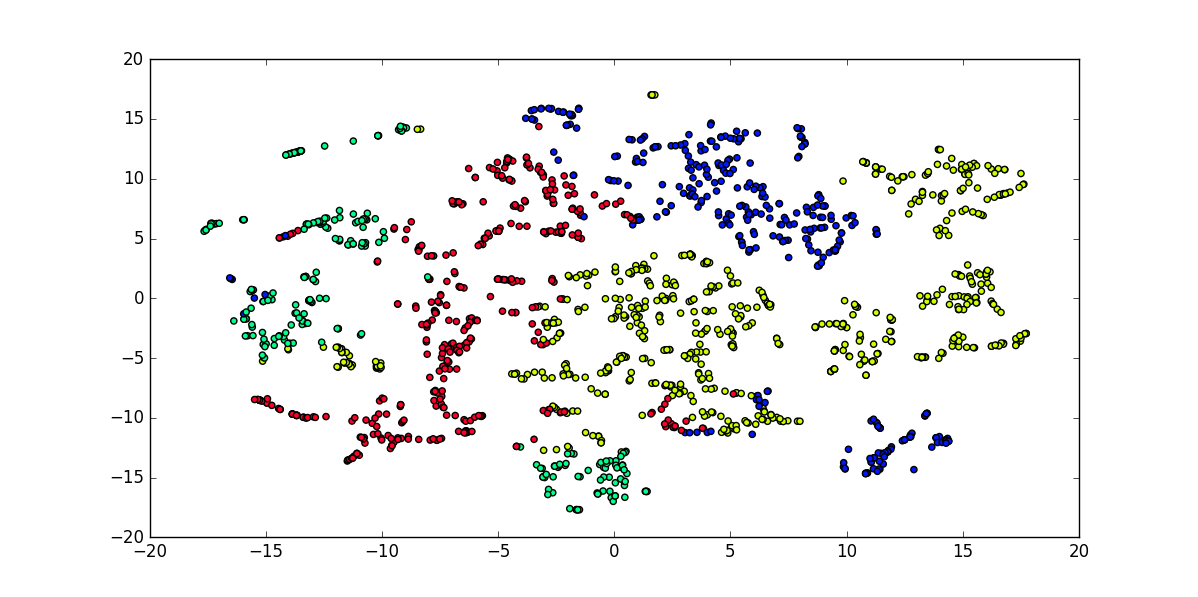
\includegraphics[width=0.5\textwidth]{../figs/consort_kmeans_2d_tsne.png}
  \caption{t-SNE visualization of K-Means with 4 clusters applied on consorting
  and consorting pairs.}
  \label{fig:consort_clustering_vis}
\end{figure}
Additionally, the centroids of the consorting clusters indicate that consorting
pairs can be clustered into:
\begin{itemize}
  \item{TODO: describe clusters}
\end{itemize}

The lower-dimensional visualization of these clusters shows cleaner separation
for the consorting pairs (Figure \ref{fig:consort_clustering_vis}) than for the
non-consorting pairs (Figure \ref{fig:non_consort_clustering_vis}).

Our initial experimentation with affinity propagation led the number of
automatically determined clusters resulted in over 64 clusters, which is too
high for us to interpret reasonably.

\subsection{Graphical Approach}

%------------------------------------------------
Of the three methods using graph theory that we implemented none performed particularly well so far. For all methods we used 5 folds of cross-validation to get test data and averaged across those folds. We always kept at least one one edge between each pair of nodes in the training data. For the latent edge prediction we got a F1 score of .08, for the latent edge prediction only using edges where one of the endpoints is one of the nodes in the test example we got a F1 score of .25. And using locally weighted regression we got an F1 score of .24. While none of these F1 scores are particularly good the more specific latent edge prediction is noteworthy in that about one third of examples there were no positive classes in the utilized training examples. This guarantees that it would predict a negative class, which would drastically hurt the F1 score. So any method to improve this, such as a back-off model that would resort to another model in these cases would be very beneficial.
\section{Next Steps}

The analysis that we have performed until now used the features directly from
the original dataset. We plan to examine if appyling additional preprocessing to
the data, such as normalizing ages or applying whitening to the derived features
can improve our algorithms.\\

The results obtained through a first pass of linear and non-linear classifiers do not measure well in terms of the defined metrics, leaving a large margin of improvement in terms of the chosen algorithms and features. Moreover, further investigation is necessary to fully understand  the reason why such algorithms have performed poorly and why they may or may not be adequate for this particular data. \\

Additionally, we plan to continue investigating clustering methods. Since we
cannot easily pick out clusters from lower dimensional representations of the
data, we are especially interested in exploring methods that can automatically
determine the number of clusters within our data, without creating an excessive
number of clusters. Some ideas are silhouette scores and graphing total cost vs. number of clusters to see if some sort of ``elbow'' exists.

For graphical analysis we will look at models that ignore many of the edge attributes and instead focus on what sort of information can be gained purely from the graph structure. Specifically we would like to adapt status and balance theory to work on bipartite graphs. While these models are unlikely to be good classifiers in and of themselves, they will utilize features that other models such as SVMs cannot see. So ensembles with SVMs and graph models are likely to provide better performance than only SVMs.

%----------------------------------------------------------------------------------------
%	REFERENCE LIST
%----------------------------------------------------------------------------------------

\begin{thebibliography}{99} % Bibliography - this is intentionally simple in this template

\bibitem[Tung et al., 2012]{Tung:2012}
  Jenny Tung, Marie J. E. Charpentier, Sayan Mukherjee, Jeanne Altmann, and Susan C. Alberts (2012)
\newblock 
  Genetic Effects on Mating Success and Partner Choice in a Social Mammal.
\newblock {\em The American Naturalist}, 2012 180:1, 113--129.

\bibitem [Macskassy,2007]{Macskassy:2007} 
Sofus A. Macskassy (2007) 
\newblock
Improving learning in networked data by combining explicit and mined links
\newblock{\em Proceedings of the 22nd national conference on Artificial intelligence}, July 22-26, 2007, p.590-595
 
\end{thebibliography}

%----------------------------------------------------------------------------------------

\end{document}
